\chapter{Evaluation}
\label{ch:evaluation}
In the evaluation chapter, we evaluate our implementation of the proposed compiler. The evaluation consists of two aspects. Firstly, we evaluate the optimizations performed by the compiler. In the second part, we evaluate the execution time and performance of the different compilation stages.

To evaluate the compiler, a program to compile is required. For this, we use the quantum ripple-carry adder proposed by Cuccaro et al.~\cite{CDKM04}. The quantum adder works similarly to its classical equivalent. For the arguments, it takes both a carry input qubit $cin$ and an output qubit $cout$ as well as two quantum registers $a$ and $b$. When applied, the adder adds the first register $a$ to the second $b$ while taking the carry input qubit $cin$ into account. If the result for the addition is larger than the register $b$, the carry output qubit $cout$ is used.
More specifically, the algorithm adds $a = a_{n-1} \dots a_{0}$ and $b = b_{n-1} \dots b_{0}$ together in place. After the computation, the resulting bit string $s = s_n \dots s_0$ is mostly contained in the $b$ register, where $b$ is now equal to $s_{n-1} \dots s_{0}$, and $s_n$ is saved in the $cout$.

To implement the ripple-carry adder, two auxiliary gates are used; these are the majority gate $\texttt{MAJ}$ and the ``unmajority and add'' gate $\texttt{UMA}$.
The \texttt{MAJ} gate computes the majority of three bits $c_i, b_i,$ and $a_i$. Together with the \texttt{UMA} gate, the result is the string bit $s_i$ in the $b_i$ register entry while the carry qubit and $a$ register are unchanged. The combined semantics and the intermediate values of the \texttt{MAJ} and \texttt{UMA} gates are depicted in Fig.~\ref{fig:eval_MAJandUMAGates}.
Their concrete implementations are given in Appendix~\ref{appendix:majGates}.
% in Fig.~\ref{fig:eval_majorityGate} and Fig.~\ref{fig:eval_unmajorityGate} respectively.  
\begin{figure}[htp!]
    %\centering
    \[
        \Qcircuit @C=1em @R=1.5em {
            & \lstick{c_i} & \multigate{2}{\text{MAJ}} & \qw & \push{ c_i \oplus a_i \hspace{1em}} & \qw & \multigate{2}{\text{UMA}} & \rstick{c_i} \qw \\
            & \lstick{b_i} & \ghost{\text{MAJ}} & \qw & \push{b_i \oplus a_i \hspace{1em}} & \qw & \ghost{\text{UMA}} & \rstick{s_i} \qw \\
            & \lstick{a_i} & \ghost{\text{MAJ}} & \qw  & \push{\hspace{.5em} c_{i+1} \hspace{1.5em}} & \qw & \ghost{\text{UMA}} & \rstick{a_i} \qw 
        }
    \]
    \caption{The combined semantics and the intermediate values of the \texttt{MAJ} and \texttt{UMA} gates.}
    \label{fig:eval_MAJandUMAGates}
\end{figure}

To compute the addition of the entire register, the \texttt{MAJ} gate is first applied to $cin$ and the first elements of the $b$ and $a$ registers. Since the intermediate carry bit is saved in the $a$ register, the \texttt{MAJ} gate is applied to each element pair of the $b$ and $a$ registers while the previous element of the $a$ register is used as the carry bit for the gate. After all \texttt{MAJ} gates are applied, the carry bit in the $a$ register is written to $cout$. Next, the \texttt{UMA} gates are applied in reversed order, similar to the \texttt{MAJ} gates. In the end, the $a$ register has the same value as before, the $b$ register contains the result of the addition, and $cout$ possibly contains an additional carry bit. The complete implementation of the adder is depicted in Fig.~\ref{fig:eval_adder_luie}.

\begin{figure}[htp]
    \centering     
    \lstinputlisting[style=Luie]{../figures/code/evaluation/adder.luie}
    \caption{A Luie implementation of a quantum ripple-carry adder circuit.}
    \label{fig:eval_adder_luie}
\end{figure}

\section{Optimization}
\label{sec:eval_optimization}
The optimizations, which are applied to the quantum circuit, are the first aspect we want to evaluate. For this, we apply our optimizations to variants of the same algorithm, the quantum ripple-carry adder. Firstly, we analyze the optimizations to the adder when given classical inputs. Next, we evaluate the optimizations of the adder for inputs in superposition with different register sizes. Lastly, we compare our optimizations to optimizations that are applied by the default Qiskit transpilation process of quantum circuits.

In our first example, we use the inputs $a = \ket{1}$ and $b = \ket{15}$, with both the input and output carry qubit having a value of $\ket{0}$. Furthermore, both input registers have a size of four qubits and, in turn, have $2^4 = 16$ possible classical values. After the adder is applied, the $a$ register and carry input, per definition, remain at their initial values of $\ket{1}$ and $\ket{0}$, respectively. In contrast, the $b$ register now has a value of $\ket{0}$ and the carry output a value of $\ket{1}$, indicating that the result of the addition is $\ket{16}$.
The quantum circuit corresponding to the example before optimization rules are applied is depicted in Fig.~\ref{fig:eval_adder_circuit}.
\begin{figure}[htp]
    \centering     
    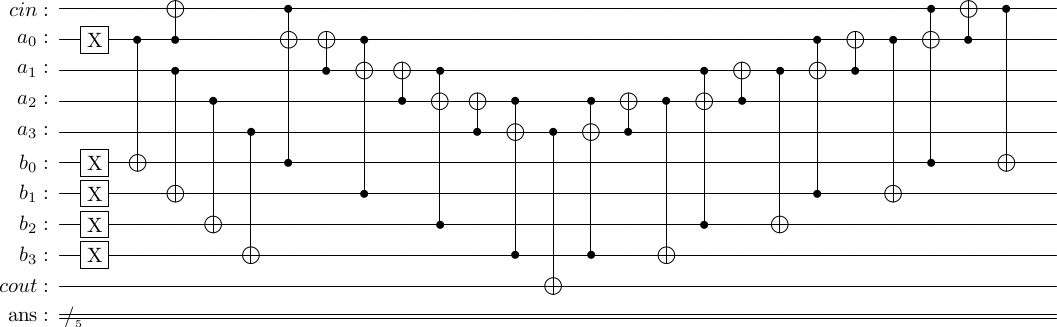
\includegraphics[width=\textwidth]{../figures/images/adderCircuit.png}
    \caption{An unoptimized circuit of a quantum ripple-carry adder.}
    \label{fig:eval_adder_circuit}
\end{figure}

Since the circuit only consists of $X$, controlled-not, and Toffoli gates, neither the Hadamard reductions nor control reversal optimization rules can be applied to the circuit. However, both the peeping control and null gate optimizations can be applied. Whenever a qubit wire contains a known value of $\ket{0}$, the controlled gates can be removed. For the opposite case, the control can be removed and the resulting $X$ gate can be removed when in combination with another $X$ gate. In turn, the circuit can be optimized such that the resulting one only contains gates that initialize the result; only two $X$ gates remain. While the first gate flips the first qubit of the $a$ register, initializing it to $\ket{1}$, the second flips the carry output qubit, indicating a result of $\ket{16}$. The OpenQASM code for the optimized circuit is depicted in App.~\ref{appendix:classicalInputs_optimized}.

In the second example, we input a value in superposition. Now, register $a$ contains a value of $\frac{1}{\sqrt{2}} (\ket{0} + \ket{3})$ and register $b$ contains a value of $\ket{4}$. Again, both carry qubits are initialized to $\ket{0}$. After the adder gate is applied, the carry qubits and register $a$ remain as initialized. However, the $b$ register now has a value of $\frac{1}{\sqrt{2}} (\ket{4} + \ket{7})$.
Since the input is now no longer a classical value, the peeping control optimization can only be applied in a few cases. In turn, only twelve gates are removed. The optimized quantum program is depicted in App.~\ref{appendix:superposInputs_optimized}. In other cases, even fewer optimizations are applied; \eg, with an input of $b = \ket{15}$, only four gates are removed while four Toffoli gates are optimized to controlled-not gates.
While the optimizations are not as effective for inputs in superposition, they can optimize significant parts of the program. For example, when we repeat both examples but increase the size of the registers to $64$ qubits, the optimized circuit contains the same amount of gates. In these cases, if qubits are not entangled by the data in superposition, all gate applications to their wires, except for the initializations, can be removed.

We also compared the optimizations applied by our compiler to the default optimizations that are applied by the Qiskit transpilation process. Qiskit\footnote{\url{https://github.com/Qiskit/qiskit/}}~\cite{JTK*24} is a software development kit for building, simulating, and transpiling quantum circuits. Additionally, the kit can interpret OpenQASM programs and build quantum circuits from them. When transpiling quantum circuits with Qiskit, \ie, transforming to a specific domain such as another basis gate set, the kit can perform optimizations to the circuit based on an optimization level. For the comparison, we used the quantum ripple-carry adder implementation provided by the OpenQASM repository\footnote{\url{https://github.com/openqasm/openqasm/blob/main/examples/adder.qasm}}. The code for the program is depicted in Fig.~\ref{fig:eval_adder_qasm}. The program can then be loaded with Qiskit and built into a quantum circuit. To apply the default optimizations of Qiskit, we transpile the circuit with the highest optimization level to the base gate set our compiler translates to, \ie, $\{X, Y, Z, CX, CCX, H\}$. While our compiler translates to arbitrary controlled gates, they are not used in this example. Furthermore, even the $Y$, $Z$, and Hadamard gates are redundant as they are not used.

\begin{figure}[htp]
    \centering     
    \lstinputlisting[style=QASM]{../figures/code/evaluation/adder.qasm}
    \caption{An OpenQASM 3 implementation of a quantum ripple-carry adder circuit.}
    \label{fig:eval_adder_qasm}
\end{figure}

However, while the Qiskit transpilation can apply many optimizations such as null gate optimizations, the default rule set does not contain a rule similar to our peeping control optimization rule. In turn, no controlled gates can be optimized in the circuit. Furthermore, since the null gate optimizations can only be applied after peeping control rules were applied, the transpilation process does not apply any optimizations to the circuit. Since Qiskit targets lower-level transpilation to specific hardware or quantum devices and not high-level optimizations, its focus is on optimizations different from ours. In contrast, our compiler has no transpilation capabilities and cannot target any specific hardware. In turn, the optimizations and overall capabilities of Qiskit and our compiler are complementary and can be used in tandem.


\section{Execution Time}
\label{sec:eval_executionTime}
The second aspect we want to evaluate is the execution time of different compilation stages. Since our compiler does not implement the lexical and syntactic analysis itself but uses ANTLR to generate the lexer and parser, our evaluation focuses on the semantic analysis, code generation, and, finally, optimization. To analyze the performance, we compiled the program with the ripple-carry adder with an input of $a = \frac{1}{\sqrt{2}} (\ket{0} + \ket{3})$ and $b = \ket{15}$. In this example, the complexity of the compiler circuit can be adjusted by changing the register sizes for $a$ and $b$. For our evaluation, we used the power of two from $16$ to $1024$. For each register size $n$, we compiled the program ten times and took the averages of the execution times for each compilation stage. The results are depicted in Fig.~\ref{tab:eval_executionTime}. 

\begin{table}[htp]
    \centering     
    \begin{tabular}{c|ccc}
    \multirow{2}{*}{Register Size $n$} & \multicolumn{3}{c}{Execution Time of Stages in ms}                                                  \\ \cline{2-4} 
                                       & \multicolumn{1}{c|}{Semantic Analysis} & \multicolumn{1}{c|}{Code Generation} & Optimization \\ \hline
                                       16                                 & \multicolumn{1}{c|}{28.3}                & \multicolumn{1}{c|}{45.4}              & 117          \\
    32                                 & \multicolumn{1}{c|}{27.5}                & \multicolumn{1}{c|}{43.8}              & 215.4          \\
    64                                 & \multicolumn{1}{c|}{27.3}                & \multicolumn{1}{c|}{47.8}              & 711.6          \\
    128                                & \multicolumn{1}{c|}{26.3}                & \multicolumn{1}{c|}{50.4}              & 2292.4         \\
    256                                & \multicolumn{1}{c|}{26.2}                & \multicolumn{1}{c|}{59.7}              & 10755.7        \\
    512                                & \multicolumn{1}{c|}{25.8}                & \multicolumn{1}{c|}{74.9}              & 60204.7        \\
    1024                               & \multicolumn{1}{c|}{26.1}                & \multicolumn{1}{c|}{109.1}             & 405376.6      
\end{tabular}
\caption{The execution times compiling a quantum ripple-carry adder with different register sizes.}
\label{tab:eval_executionTime}
\end{table}

The first stage is the semantic analysis. In this stage, the source code is analyzed for semantic error such as undeclared variables or type errors. Since the analysis is performed on the source code, the execution time does not change significantly with a change in register size, as the source code size and complexity remains unchanged. The value range from $25.8$ ms to $28.3$ ms with an average of $26.79$ ms. 

Next, the code generation stage generates the target code from the source code. In our example program, the source code size stays constant. Both the \texttt{MAJ} and \texttt{UMA} gates are not dependent on the register size. However, the adder gate iterates over the size of the registers twice. In turn, the generated code size increases linearly with an increase in register size. This trend is not clear for small register sizes between $16$ and $64$. However, for larger register sizes, a linear trend is visible.

Lastly, the optimizations stage applies optimization rules, if possible, to the generated quantum circuit and, thereby, reduces its complexity. The optimization algorithm iterates over the circuit by going through all qubits. From there, it iterates over all gates on the qubit wire. In the case that all gates operate on all qubits, the resulting circuit iteration has a complexity of $n_g \cdot n_q$ where $n_g$ and $n_q$ are the number of gates and qubits respectively. Additionally, the circuit iteration is repeated as long as optimizations can be found. In the case that all gates can be optimized and are only optimized one at a time, the overall complexity of the optimization is $n_g^2 \cdot n_q$. Since the number of gates increases linearly with the register size in our example, the worst case complexity for its optimization is $\mathcal{O}(n^3)$ where $n$ is the register size. While the worst case would be a cubic increase in execution time when increasing the register size, the data shows an approximate quadratic increase, starting at $117$ ms on average for a register size of $16$ and going up to about $6$ minutes and 45 seconds for a register size of $1024$. 



